\documentclass{article}

\title{The numeric tower fiasco}
\subtitle{Inheritance is scam}
\date{2023-11-22}
\modified{2023-11-22}
\keyword{oop}

\begin{document}

\epigraph{Object-oriented programming is an exceptionally bad idea which could only have originated in California.}{Edsger Dijkstra}

\section{introduction}{Introduction}

Object-oriented programming\sidenote{sn-oop}{
    ``Object-oriented'' is a vague term that means different things to different people.
    This article focuses on the class-based flavor that the most popular programming languages (Java, Python, C++, C#) implement.
} is still the dominant paradigm in the software industry.
The typical advice on modeling the problem domain is to fit your entities into hierarchies where specific types inherit common attributes and behaviors from ``base'' classes.

That idea looked intuitive and attractive to me when I first encountered it.
I spent countless hours learning about the ``good'' object-oriented design and trying to apply these ideas in practice.

The practice showed that real engineering problems rarely fit into rigid class hierarchies.
I grew more frustrated with object-oriented programming and eventually entirely gave up on it.
This article describes one example that stuck with me from the start of my programming career: modeling the hierarchy of number types.

\section{the-numeric-tower}{The numeric tower}

\epigraph{God made the integers, all the rest is the work of man.}{Leopold Kronecker}

I like math, so one of the first structures I tried to model with classes was the most precisely specified and well-studied hierarchy in human history: the \href{https://en.wikipedia.org/wiki/Numerical_tower}{numerical tower}.

Mathematicians discovered\sidenote{sn-motivation}{
  The primary motivation for introducing integers was to create a numeric space where equations of the form \math{a + x = c}, where \math{a} and \math{c} are naturals, always have a solution.
  Rationals play the same role for equations of the form \math{a × x = c}.
} quite a few types of numbers; usually, each new type is the most natural extension of the previous one:

\begin{itemize}
  \item Naturals (\math{ℕ}) are the numbers we use for counting: \math{0, 1, 2, \ldots}.
  \item Integers (\math{ℤ}) extend naturals to include negative whole numbers: \math{0, 1, -1, 2, -2, \ldots}.
  \item Rational numbers (\math{ℚ}) add common fractions where the numerator and denumerator are whole numbers: \math{1}, \math{½}, \math{-½}, \math{⅓}, \math{-⅓}, \ldots.
\end{itemize}

\begin{figure}[grayscale-diagram,medium-size]
  \marginnote{mn-numeric-tower}{
    A few floors of the \href{https://en.wikipedia.org/wiki/Number}{numeric} tower represented as a \href{https://en.wikipedia.org/wiki/Venn_diagram}{Venn diagram}.
  }
  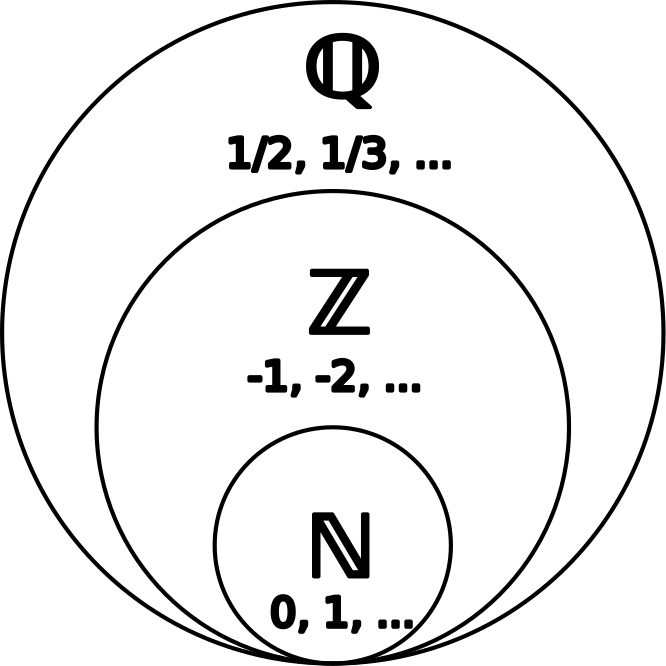
\includegraphics{/images/23-numeric-tower.svg}
\end{figure}

The tower goes up and includes real numbers, complex numbers, quaternions, etc.

\section{oop-design}{The OOP design}

In this section, we'll design a class hierarchy modeling the numbers using an imaginary object-oriented programming language.
We'll limit the tower to only two number types to keep the example simple: \code{Naturals} and \code{Integers}.

Most people (me included) will instinctively reach for the class structure where \code{Natural} is the base class, and \code{Integer} extends that base.

\begin{figure}
\marginnote{mn-nat-base-hierarchy}{
  Pseudocode of a class hierarchy in which the \code{Natural} class is the base and the \code{Integer} class extends it.
}
\begin{code}[pseudo-code]
class Natural
  value : UInt

  def make(value : UInt) : Natural = \ldots
  def +(other : Natural) : Natural = Natural.make(self.value + other.value)
end

class Integer <: Natural
  negative? : Bool

  def make(value : Natural, negative? : Bool) : Integer = \ldots
  def magnitude() : Natural = self.value
  def +(other : Integer) : Integer = \ldots
end
\end{code}
\end{figure}

I'm sure you immediately spotted a problem with this design: we inverted the hierarchy, breaking the ``is a'' relationship!
We claim that all integers are also naturals, but that's false.
The design violates the \href{https://en.wikipedia.org/wiki/Liskov_substitution_principle}{Liskov substitution principle}: passing an \code{Integer} to a function that expects a \code{Natural} can produce incorrect results:

\begin{code}[pseudo-code]
> Natural.make(5) + Integer.make(10, true) // 5 + -10
15 // ouch
\end{code}

Enlightened by this failure, we reverse the inheritance hierarchy.
\code{Integer} becomes our base class, and \code{Natural} extends it.

\begin{figure}
\marginnote{mn-integer-base}{
  Pseudocode of a class hierarchy in which the \code{Integer} class is the base and the \code{Natural} class extends it.
}
\begin{code}[pseudo-code]
class Integer
  value : UInt
  negative? : Bool

  def make(value : Natural, negative? : Bool) = \ldots
  def magnitude() : Natural = self.value
  def +(other : Integer) : Integer = \ldots
end

class Natural <: Integer
  def make(value : UInt) : Natural = super.make(value, false)
  def +(other : Natural) : Natural = \ldots
end
\end{code}
\end{figure}

Once the initial excitement dissipates, we face a new issue.
The simplest case, the \code{Natural} numbers, must have the same representation as the more complex type, \code{Integers}.
The problem becomes more apparent if we add more types to the tower, such as \code{Rational}.
Instead of starting with the simplest case and building from it, we started with the most complicated one and made everything else a special case.
That's why the original incorrect design was so compelling: we moved from simpler to more complex types, not the other way around!

Another design option is to give up concrete type hierarchies and clamp all number types under a single interface.

\begin{figure}
\marginnote{mn-number-interface}{
  Pseudocode of a type hierarchy where all numeric types implement the same interface.
}
\begin{code}[pseudo-code]
interface Number
  def +(n : Natural) : Number
  def -(n : Natural) : Number
  // \ldots
  def +(i : Integer) : Number
  def -(i : Integer) : Number
  // \ldots
end

class Natural <: Number
  // a lot of boring code \ldots
end

class Integer <: Number
  // a lot of boring code \ldots
end
\end{code}
\end{figure}

This approach is the most versatile, but it has many drawbacks:
\begin{itemize}
  \item The programmer must write a lot of boilerplate code.
  \item All types in the hierarchy need to know about one another.
  Adding a new type requires changing all other types.
  \item Adding a new operation on numbers requires modifying all the classes.
\end{itemize}

It's time to abandon our blunt OOP tools and start from the first principles.

\section{the-functional-design}{The functional design}

The object-oriented tradition obsesses with encoding ``is a'' relations among types as a class hierarchy.
In this section, we'll use the approach mathematicians employ: we start with simple structures and combine them to form more complex objects.
This approach is similar to using composition instead of inheritance in the OOP world.

Our tool of choice will be the \href{https://haskell.org/}{Haskell} programming language, but the same principles will work in all languages supporting \href{https://en.wikipedia.org/wiki/Algebraic_data_type}{algebraic data types} and functions (even \href{https://www.rust-lang.org/}{Rust} would do, though it would be less pretty).

In our first attempt, we will model each numeric type with a separate Haskell type.

\begin{figure}
\marginnote{mn-functional-nums}{
  Modeling the \code{Natural} and \code{Integer} numeric types in Haskell.
}
\begin{code}[haskell]
-- Each natural is either zero or a successor of a smaller number.
data Natural = Zero | Succ Natural -- \circled{1}

-- There are two disjoint classes of integers:
-- \math{n} and \math{-1 - n} for all natural values of \math{n}.
data Integer = NonNegative Natural | MinusOneMinus Natural -- \circled{2}

-- We model the `is a' relation as a pure total function
-- mapping naturals to integers.
int_of_nat :: Natural -> Integer -- \circled{3}
int_of_nat = NonNegative

-- We can model the reverse relation as a partial function
-- mapping integers to naturals.
nat_of_int :: Integer -> Maybe Natural
nat_of_int (NonNegative n) = Just n
nat_of_int (MinusOneMinus _) = Nothing

plus_nat :: Natural -> Natural -> Natural
plus_nat n Zero = n
plus_nat n (Succ m) = Succ (plus_nat n m)

plus_int :: Integer -> Integer -> Integer
plus_int = \ldots

minus_int :: Integer -> Integer -> Integer
minus_int = \ldots
\end{code}
\end{figure}

\begin{enumerate}
  \item
    According to \href{https://en.wikipedia.org/wiki/Peano_axioms}{Peano}, a natural number is either a zero or a successor of a smaller natural number.
    This definition is equivalent to the \href{https://en.wikipedia.org/wiki/Unary_numeral_system}{unary numeral system}, which is inefficient for computation but convenient for demonstration.
  \item
    An integer number is either a non-negative natural number \math{n} or a negative number \math{-1 - n}, where \math{n} is a natural number.
    Note that with this definition, each integer has a unique representation.
  \item
    We encode the ``is a'' relation between numeric types as a pure total function.
    OOP languages usually generate these type-casting functions automatically and apply them implicitly.
\end{enumerate}

Note how modular this implementation is.
Naturals can live in a separate module and don't need to know about the existence of integers.
We can easily change the implementation of naturals (e.g., use the more efficient \href{https://en.wikipedia.org/wiki/Binary_number}{binary representation}) or add more numeric types (e.g., \code{Rational}s) without breaking other code.

However, the design is not yet satisfactory: we lost the ability to operate uniformly on numbers of different types.
We can add a universal \code{Number} type to reclaim this property.

\begin{figure}
\marginnote{mn-universal-number}{
  Modeling the numeric tower in Haskell with a sum type.
}
\begin{code}[haskell]
-- The sum type encoding all number types.
data Number = Nat Natural | Int Integer

-- Adds arbitrary numbers.
plus :: Number -> Number -> Number
plus = \ldots

-- Subtracts arbitrary numbers.
minus :: Number -> Number -> Number
minus = \ldots
\end{code}
\end{figure}

This design might seem like a re-iteration of the \code{Number} interface story from the OO world, but it's not:

\begin{itemize}
  \item
    We have many opportunities to reduce the boilerplate code to the bare minimum.
    We will discuss these opportunities shortly.
  \item
    The module implementing \code{Naturals} doesn't need to know about \code{Integers} or \code{Numbers}.
  \item
    We don't need to modify existing types when we add new functions operating on numbers.
\end{itemize}

To address the boilerplate issue, we'll introduce the numeric type \em{promotion} operation.
When we add two numbers of different types, we convert the simpler type to the more complex one using the previously discussed type conversion functions.
We then apply the binary operator dealing with numbers of the same promoted type.
Finally, we demote the result to the simplest type that can hold the value.

\begin{figure}
\marginnote{mn-universal-number}{
  Reducing the boilerplate with type promotion.
}
\begin{code}[haskell]
data Number = Nat Natural | Int Integer

-- Promotes the arguments to the largest common type.
promote :: (Number, Number) -> (Number, Number)
promote (Nat n, Int m) = (Int (int_of_nat n), Int m) 
promote (Int n, Nat m) = (Int n, Int (int_of_nat m))
promote x = x

-- Reduces the number to its most canonical form.
simplify :: Number -> Number
simplify (Int (NonNegative n)) = Nat n
simplify x = x

type BinaryOp = Number -> Number -> Number

-- Implements a total binary operation given a kernel defined
-- only on numbers of the same type.
impl_binary_op :: BinaryOp -> BinaryOp
impl_binary_op kernel x y = let (x', y') = promote (x, y)
                            in simplify (kernel x' y')

-- Adds arbitrary numbers.
plus :: Number -> Number -> Number
plus x y = impl_binary_op plus_simple x y
  where plus_simple (Nat n) (Nat m) = Nat (plus_nat n m)
        plus_simple (Int n) (Int m) = Int (plus_int n m)
        plus_simple _ _ = undefined

-- Subtracts arbitrary numbers.
minus :: Number -> Number -> Number
minus x y = impl_binary_op minus_simple x y
  where minus_simple (Nat n) (Nat m) = Int (minus_int (int_of_nat n) (int_of_nat m))
        minus_simple (Int n) (Int m) = Int (minus_int n m)
        minus_simple _ _ = undefined
\end{code}
\end{figure}

The \code{impl_binary_op} function captures the promote/execute/simplify pattern.
Concrete binary operators (\code{plus}, \code{minus}, etc.) must deal only with numbers of the same type.

With this, we get a clean and concise model of numbers on a computer.
The code is easy to extend to support more numeric types, which is left as an exercise for the reader\sidenote{sn-complex}{
  I find adding the \code{Complex} type particularly interesting.
  Hint: you might need two different generic \code{Number} types.
}.

\section{conclusion}{Conclusion}

\epigraph{I find OOP technically unsound\ldots  I find OOP philosophically unsound\ldots  I find OOP methodologically wrong.}{From \href{http://stlport.org/resources/StepanovUSA.html}{An Interview with A. Stepanov}}

When I use a tool and get unsatisfactory results, I blame myself for not using the tool correctly.
At first, I felt the same about the numeric tower case, but now I'm sure the problem is not me; it's the class hierarchies.

The approach of piling classes on top of one another and trying to make this stack coherent is fundamentally flawed.
It fails spectacularly even on tiny examples where the problem domain is \em{mathematically} specified.
The numeric tower is one example, but there are more.
The \href{https://en.wikipedia.org/wiki/Circle%E2%80%93ellipse_problem}{circle-ellipse problem} is a good one,
but my favorite is how inheriting \code{ColorPoint} from \code{Point} breaks the transitivity property of the \code{equals} method:

\blockquote{
    There is no way to extend an instantiable class and add a value component while preserving the \code{equals} contract,
    unless you're willing to forgo the benefits of object-oriented abstraction.
}{Joshua Bloch, ``Effective Java'', 3rd edition, item 10, p. 42}

If something doesn't work on small examples, why do we expect it to work in large codebases?
When was the last time you looked in a complex class hierarchy and admired how easy to understand the code was?

Experts often recommend ``favor composition over inheritance''\sidenote{sn-composition-over-inheritance}{
  E.g., Joshua Bloch, ``Effective Java'', third edition, item 18, p. 87.
}.
I agree with them and favor algebraic data types and simple functions as the ultimate form of composition.

\end{document}